\chapter{Introduction} \label{ch:introduction}

April 12 deadline- two passes (a week each) gives us roughtly last week of march for rough draft.  Look up correlation coefficient //

A Genetic Algorithm (GA) is a biologically inspired form of computing.  GAs can be used for many different purposes, from optimization to classification to design and testing.  They can be applied anywhere that a solution can be encoded and then autonomously evaluated.  However, they are most well understood as a general solution to optimization as a form of stochastic gradient descent, similar conceptually to simulated annealing. In this paper, I attempt to narrow the role of GAs as they pertain to pattern recognition and classification.  In the remainder of this chapter I will describe GAs in general terms and discuss the motivations of this paper.  In chapter 2, I will discuss the specifics of the GAs which I use in this paper in detail.  In chapter 3 I will describe the experiments conducted and discuss the results.  In Chapter 4 I will describe future avenues of study which are available. 
\paragraph{Genetic Algorithms Introduction}
Imagine a colony of rabbits.  The rabbits are quite content to munch on clovers and thistles and the like.  Some rabbits are much more content than others, and have significant girth.  One day foxes find the rabbits. There are many more rabbits than foxes, and the foxes can't eat all of them.  The heaviest rabbits are both the slowest and the most appetizing to the foxes, and they are the first to go, but many die.  They have failed the evolutionary filtering process.  However, the rabbits that survive are thinner, and the most successful are likely faster.  These are the rabbits which survive to populate the next generation.
\\GAs encapsulate this process, though usually with much less mayhem.  The algorithm is as follows:
\begin{lstlisting}[language = algorithm]
Population := RandomInitialization()
	while True:
		For each Solution in Population:
			Evaluate Solution
			Assign Fitness to Solution
		newPopulation = SurviveAndBreed(Population)
		Population = newPopulation
	end while
\end{lstlisting}

\subparagraph{Stopping Conditions} This algorithm can run for a predetermined number of generations, indefinitely, or until another specific criteria is met.  Consider the problem of finding a way of combining 4 operands with 3 operators to achieve a particular value.  There are often many ways to solve this problem.  If one was to use a GA to solve the equation, the algorithm could stop as soon as it had a valid solution values for a, b, c, d, and the 3 operators which satisfied the equation.  For example:
\begin{align*}
		a \: op_1\: b\: op_2\: c\: op_3\: d &= x\\
		3 \times 7 \times 3 + 5 &= 68\\
		9 \times 7 + 8 - 3 &= 68
\end{align*}
\subparagraph{Solution Encodings}
Now lets look specifically at what is meant by a solution.  First, GAs usually have some encoding based ultimately on a string of 0s and 1s, called a bitstring\footnote{Other genetic alphabets are possible as well, though less common.}. Continuing with our example, we know that there are 4 operands which have a value between 0 and 9, or 10 values total.  To encode that in a bitstring we use the values 0000-1010.  We could also include some error correcting code to randomly reassign the bits if they go outside of the values, ensuring that any solution randomly generated contains valid data (we could also use more bits and/or arbitrarily assign values via modulo arithmetic, but this is the most instructive method for our current purposes).  Next, we have the operators, which can be $+$, $-$, $*$, $/$.  These fit nicely within the 00-11 bit range, with no need of error correction.  So we have a bitstring with the form xxxx-xx-xxxx-xx-xxxx-xx-xxxx\footnote{We use the hyphens here only for readability- the bitstrings contain only 1s and 0s.}, 22 bits which satisfy the constraints of our problem. The second line of the above example would be 0011-10-0111-10-0011-00-0101.
\subparagraph{Fitness Functions}
Following along with the algorithm, we need to assign fitness.  In this case the closer one is to the solution, the better, usually \footnote{There are examples of x where this won't work as well- in a shortened version of our example problem, for instance, if the target is 25, $2\times3\times4$ will quickly dominate the fitness landscape but isn't actually any closer to a valid solution than $5\times5+9$.}.  There is research showing that a fitness function should be differentiable, at least as far as the solution space.  Point discontinuities aren't an issue if they occur outside of the solution space, which is important for us because we're going to make use of one. Specifically, the function 
\begin{equation*}
F(s) = \frac{1}{|E(s)-x|}
\end{equation*}
Where E(s) is the result returned by evaluating s, the numeric string.  So if we had the string 3-6*6+2, then E(s)= -16.  Assuming x is still 68, then the fitness for that particular s would be \(\frac{68}{84}= 1.19E-2\), extremely low. When 
E(s) = x or F(s) = ${\infty}$
we break out of the infinite loop.  This would be a discontinuity, but the function is still differentiable across where we're evaluating it.
\subparagraph{Breeding and Survival}
Now that we have a fitness function, we can evaluate the entire population and determine who has the highest fitness.  With a random seed, the first generation is usually not very fit.  Regardless, the next step is to see who survives and who breeds into the next generation.
Survival is usually an arbitrary matter of copying the best solution(s) \textit{in toto} to the next generation.  \footnote{Some variations have ages, where all solutions will live a certain amount of time, and more fit solutions have longer lifespans than less fit solutions.  These will not be covered further in this document.}  This is typically referred to as elitism, and it is usually a percentage around 10\% of the population that is uncritically copied into the next generation.  Properly done, this guarantees monotonically non-decreasing fitness of the best solution from one generation to the next.\\
The next step is to pick some fraction of the population as breeding stock.  The most fit are generally given preferential treatment, but not exclusive preference.  This is in large part because in GAs as in life, genetic diversity is a critical trait to the overall fitness of a population.  For GAs, it means that diversity speeds convergence to ensure that even the less fit have a chance to propagate into the next generations.  The method we employ, a fairly standard one, is Roulette Uniform Selection.  To get an intuition for the algorithm, see ~\ref{fig:rusillustration}.  In it, you can see that RUS chooses markers (represented by the arrows) equally spaced between the beginning of the population and the end.  Everywhere a marker falls means a copy of that solution gets passed into the breeding population for the next generation.  This is usually guaranteed to get at least 1 copy of the most fit individual, but everything else is based on chance.  
\begin{figure}
	\centering
	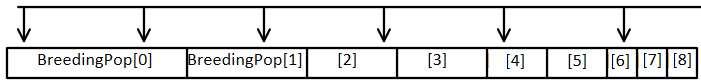
\includegraphics[width=0.7\linewidth]{figures/png/RUSIllustration}
	\caption[Roullete Uniform Selection]{An example of RUS. The bar represents the cumulative fitness of the population. The arrows represent which members of the population go on to become a breeding member.  In this example, 3 gets skipped even though it has higher fitness than 4 and 6, while 0 gets copied into the breeding population twice.}
	\label{fig:rusillustration}
	
\end{figure}
\\
With a breeding population in place, we can begin the breeding process.  This is typically accomplished via an operation called crossover, which I will explain below.  \\\begin{tabular}{c|c|c|c|c|c|c|c|}
	\textit{A} & \textit{1001} & \textit{10} & \textit{0011} & \textit{11} & \textit{1001} & \textit{00} & \textit{0111}\\ 
\textbf{B} & \textbf{0011} & \textbf{01} & \textbf{1000} & \textbf{01} & \textbf{0001} & \textbf{10} & \textbf{1001}\\
	
\end{tabular}\\
We begin with two solutions.  Crossover takes and returns 2 bitstrings.    It also has several subtypes, which I will illustrate in sequence.  First is one-point crossover.  This means that before crossing, a crossover point is chosen and offspring are produced as a copy, and when this point is reached, the offspring cross over and begin taking material from the other parent.  \\

\begin{tabular}{c|c|c|c|c|c|c|c|}
	\textit{A'} & \textit{1001} & \textit{1}\textbf{1} & \textbf{1000} & \textbf{01} & \textbf{0001} & \textbf{10} & \textbf{1001}\\ 
	\textbf{B'} & \textbf{0011} & \textbf{0}\textit{0} & \textit{0011} & \textit{11} & \textit{1001} & \textit{00} & \textit{0111}\\
	
\end{tabular}\\

Two point crossover is similar to one point, except that crossing happens twice.\\

\begin{tabular}{c|c|c|c|c|c|c|c|}
	\textit{A'} & \textit{1001} & \textit{10} & \textit{00}\textbf{00}  & \textbf{01} & \textbf{0001} & \textbf{10} & \textbf{1}\textit{111}\\ 
	\textbf{B'} & \textbf{0011} & \textbf{01} & \textbf{10}\textit{11} & \textit{11} & \textit{1001} & \textit{00} & \textit{0}\textbf{001}\\
	
\end{tabular}\\

Notice that here the final digit of A' and the second digit of B' becomes invalid (1111 is not between 0000 and 1001)- this is not controlled for in Crossover, but rather handled later by evaluating the offspring.

The final standard type is uniform crossover, which makes a check at each bit to crossover.  It results in much more mixing, depending on the probability of a crossover event.  One advantage is that it treats the beginning and end as the same, which can't be said for either of the first two.  Another is that it allows the designer to specify, directly and exactly, how much gene mixing should occur on average.

One thing that might be noticed is that regardless of where the crossover point is, with these methods if both A and B contain a particular bit in the same location, it will appear in both offspring.  This is one reason that diversity is important- if the population becomes too homogeneous, it will be unable to change except through random mutation, which we discuss shortly.\\
One other form of crossover we will deal with is one that counters this potential vulnerability.  It is a shifted crossover, so that one bitstring shifts forward a random number of bits, and then crossover proceeds normally.
\\
Other forms of crossover are possible, though they are not as widely represented in the literature.  One is a modified uniform crossover that checks to cross only  at each "word", that is at each column representing a digit or operator in our example.  This gives the designer some control over how much contiguous information is exchanged per crossover.  Other variations with three or more parents, or even random asexual reproduction are possible.  Logical operations are viable, though again care must be taken to not increase homogeneity overmuch. \\

\subparagraph{Mutation}
Mutation is fairly straightforward.  Usually after crossover and before insertion in the next generation, that is, only affecting the offspring of breeding and not elitism, each bit in the bitstring has a chance to change.  The algorithm is perhaps the most instructive: \begin{lstlisting}
for (Solution s in Crossover(A,B)):
	For bit in s.Bits:
		if(MutationChance > Random(0,1)) bit = !bit
	end for
end for
\end{lstlisting}
There are some implementations that vary in that they will change random values to 1 or 0 rather than flipping bits (in other words, values will change about half as often).  A standard value for mutation is small, about 
${\frac{1.0}{Solution.Length}}$ which means on average 1 bit will change per solution per generation.\\
What is less straightforward are the effects of mutation over a population.  While values of 0 often stagnate in local minima, an upper correlate doesn't seem to exist- one could set mutation high, say 25\%, and turn off crossover entirely, and proceed with elitism and mutation alone and arrive at solutions.  In practice, this is much slower than using crossover. A general rule of thumb is to keep mutation low, and increase it even more slowly to combat stagnation.\\
\paragraph{Drawbacks}
While GAs have great versatility, there are some drawbacks which significantly limit their utility.
\subparagraph{Swiss-Army Chainsaw}
First, GAs are not the perfect solution for anything.  At their core, they are a biased-walk\footnote{With a random-walk on one side of the spectrum and a guided approach on the other.}.  This means that while they will come to a local optima, there is no guarantee they will achieve a global optimum.  If there exists a tailored solution for a problem, using that will probably work faster and better.
\subparagraph{And Quick to Anger}
Second, GAs are subtle things.  The fitness function, not given its due in this writeup, can be the difference between a quickly converging solution and processors spinning their wheels for days or months coming to one sub-satisfactory solution after another.  A GA will optimize the fitness function- and that's all it will do.  So if you want to maximize a metric, say accuracy for a classifier, be aware that it might do exactly that by simply guessing the most prevalent answer in the dataset.  This will get it to a local optima, and it might be surprisingly difficult to get it out of it.\\
Furthermore, there are hyperparameters which effect the GA directly but can be difficult to tease out.  What should the elitism percent be?  It probably depends on your other parameters.  There are ways of optimizing these, and they themselves might be amenable to a further GA, except that evaluating them is time consuming- should your fitness function be speed of convergence?  Or the best solution arrived at within 100 generations?  That might seem too long, but use fewer generations and you run the risk of invoking too much sensitivity to starting conditions to draw meaningful conclusions.  There are some rules of thumb to assist with these situations, but they only mitigate the problem, they don't eliminate it entirely.
\subparagraph{Toolset}
Finally, a GA is only as good as its toolbox.  On Earth, that toolkit was physics.  All of physics, and massively, embarrassingly parallel at that.  That's difficult to take advantage of digitally, where you not only have the responsibility of developing an encoding but also defining the universe your population lives in.  For instance, the heart of this paper is whether to use a GA to optimize a classifier or to use a GA to classify things.  The classifier has theory underpinning its toolkit, the GA has only whatever fitness function and encoding it is supplied.  Or, to get back to our example, it might speed convergence to increase mutation rates and restrict crossover to occur only at the breakpoints of binary words.  The downside of this is that GAs are supposed to be able to solve any problem, and while they can, they also require a certain amount of customization to not waste everyone's time.  The harder the problem, the more customization that is usually required.  And at that point, if a tailored solution of some kind exists it's probably easier to code up and implement than an equivalent GA.  At their core, the GA is a biased walk, but building in paths will hopefully make that walk much quicker.
\paragraph{Theoretic Underpinnings}
Holland's Schema theorem.  
\pagebreak
